\documentclass[11pt,a4paper]{article}
\usepackage[margin=20mm]{geometry}
\usepackage[T1]{fontenc}
\usepackage{lmodern}
\usepackage{graphicx}
\usepackage{booktabs,longtable,tabularx,array}
\usepackage[dvipsnames,table]{xcolor}
\usepackage{hyperref}
\usepackage{listings}
\usepackage{enumitem}
\usepackage{fancyhdr}
\usepackage{microtype}
\usepackage{caption}
\hypersetup{colorlinks=true,linkcolor=NavyBlue,urlcolor=MidnightBlue,citecolor=NavyBlue}
\setlength{\parindent}{0pt}
\setlength{\parskip}{5pt}
\renewcommand{\arraystretch}{1.18}
\definecolor{B4Blue}{HTML}{1F4E78}
\definecolor{B4Light}{HTML}{EAF2F8}
\definecolor{B4Green}{HTML}{2F855A}
\definecolor{B4Amber}{HTML}{9C6500}
\pagestyle{fancy}
\fancyhf{}
\lhead{B4 - Property Rental Application}
\rhead{Design Pattern Case Study}
\cfoot{\thepage}
\setlength{\headheight}{14pt}
\lstset{basicstyle=\ttfamily\scriptsize,breaklines=true,frame=single,rulecolor=\color{gray!45},numbers=left,numberstyle=\tiny\color{gray},xleftmargin=1.5em,showstringspaces=false,tabsize=4}
\newcommand{\codepath}[1]{\path{#1}}
\newcommand{\statuspending}{\textcolor{B4Amber}{\textbf{Pending human input}}}

\begin{document}

\begin{titlepage}
\centering
\vspace*{18mm}
{\Large 23CSE455 Design Patterns\par}
\vspace{8mm}
{\Huge\bfseries Design Pattern Identification and Evolution\par}
\vspace{3mm}
{\LARGE in a Laravel-Based Property Rental Application\par}
\vspace{16mm}
{\Large Team B4\par}
\vspace{8mm}
\begin{tabular}{ll}
Earlapally Sahith Siddarth & Roll number: AM.SC.U4CSE23217; Batch: 2\\
Bussa Surya & Roll number: AM.SC.U4CSE23213; Batch: 2\\
Eati Manoj & Roll number: AM.SC.U4CSE23317; Batch: 2\\
Kankanala Sanithya Reddy & Roll number: AM.SC.U4CSE23327; Batch: 2\\
\end{tabular}
\vfill
\begin{minipage}{0.88\textwidth}
\small
\textbf{Submission status.} The technical report, source snapshots, diagrams, tests, four-language implementations, prompts, CSV files, and Excel workbook are complete.
\end{minipage}
\vfill
{\large 11 October 2026\par}
\end{titlepage}

\pagenumbering{roman}
\setcounter{tocdepth}{1}
\tableofcontents
\clearpage
\pagenumbering{arabic}

\section{Executive summary}

This case study examines the public MIT-licensed \emph{Property Management} Laravel application by Mohsin Rafique at baseline commit \codepath{f127b4e218018715586a52cede08e182ca45c983}. The inspected Laravel 12 source implements property, owner and tenant management, authentication, role authorization, rent/payment receipts, security deposits, and Blade views. Five baseline collaborations are confirmed: Model-View-Controller (MVC), Active Record, Chain of Responsibility, Template Method, and Laravel Facade. Repository, Strategy, and Observer claims were rejected at baseline because the application directly uses Eloquent, declares no interchangeable business algorithm, and has no application notification collaboration.

Three changes evolve that preserved baseline. CH01 introduces Strategy for dynamic pricing and integrates it with rent-receipt creation. CH02 introduces Specification for composable property filters and integrates request-driven filters with the property controller. CH03 introduces State plus an Eloquent model and migration for digital contracts. The cumulative design has eight distinct pattern types and eight pattern instances. Production PHP under \codepath{app/} grows from 2,055 to 2,450 physical LOC. The final Laravel suite passes 2/2 and the focused evolution runner passes 10/10. The unchanged upstream baseline has one passing test and one stale example test that expects HTTP 200 even though the root route intentionally redirects to login; this discrepancy is preserved as evidence and corrected only in the evolved snapshot.

The two most significant evolution patterns, Strategy and Specification, are implemented against identical fixtures in Java, Python, JavaScript, and C++. All Strategy variants pass 6/6 checks; all Specification variants pass 5/5. One warmup and five measured processes were run after compilation where applicable. The measured medians include runtime startup and test execution, so they are reproducibility evidence rather than a universal performance ranking.

\section{Application description and framework architecture}

\subsection{Application and source identity}

The selected application is \emph{Property Management}, available at \url{https://github.com/mohsin-rafique/property-management}. The baseline is upstream commit \codepath{f127b4e218018715586a52cede08e182ca45c983}, dated 1 September 2026 and accessed 11 October 2026. The repository declares the MIT license. The exact source without Git metadata, dependencies, or environment secrets is preserved at \codepath{Part1/code}; the cumulative evolved source is preserved at \codepath{Part2/code}.

The public application targets PHP 8.2+ and Laravel 12, uses Eloquent with MySQL/MariaDB, Blade views, Laravel UI authentication, role middleware, and DomPDF. The baseline and final source manifests provide integrity evidence. Local evolution commits preserve each change:

\begin{tabular}{@{}ll@{}}
CH01 & \codepath{7e9bd9ded113e91cca10e727a7eeff29c88d0ed8}\\
CH02 & \codepath{2b2dd6246dd50f4a53a991e5429b22da1b1a5c4f}\\
CH03 & \codepath{8e2af082067bb83aab7e40caf2b7a463fef8b643}\\
Verification & \codepath{27b78c16c897c845efe052101e7f47f2ad7c25cf}\\
\end{tabular}

Faculty approval remains a human-only confirmation and is not fabricated.

\subsection{Functional scope}

\begin{longtable}{p{0.19\textwidth}p{0.33\textwidth}p{0.38\textwidth}}
\toprule
\rowcolor{B4Blue}\color{white}\textbf{Area} & \color{white}\textbf{Primary symbols} & \color{white}\textbf{Observed responsibility}\\
\midrule
Property management & \codepath{Property}, \codepath{PropertyController}, Blade views & Create, view, update, delete, paginate, assign owner/tenant, and track vacancy.\\
Owner management & \codepath{Owner}, \codepath{OwnerController} & Create owner accounts and expose owner-property relationships.\\
Tenant management & \codepath{Tenant}, \codepath{TenantController}, tenant dashboard & Create tenant accounts, assign properties, and expose tenant receipts.\\
Property search & \codepath{PropertyController::index} & Baseline pagination; evolved address, rent, status, and composable domain specifications.\\
Lease management & Property tenant assignment; no baseline lease entity & Baseline records occupancy but lacks a dedicated lease. CH03 adds digital-contract state and persistence.\\
Payment & \codepath{RentReceipt}, electricity and maintenance receipts & Record rent and utility/maintenance payments and generate PDFs.\\
Notification & \codepath{User::Notifiable}; no application notification workflow & Framework capability is present, but no baseline Observer collaboration is claimed.\\
Authentication / authorization & Laravel UI controllers, \codepath{auth} and \codepath{RoleMiddleware} & Authenticate users and restrict tenant, owner, and administrator routes.\\
\bottomrule
\end{longtable}

\subsection{Architecture}

\begin{figure}[htbp]
\centering
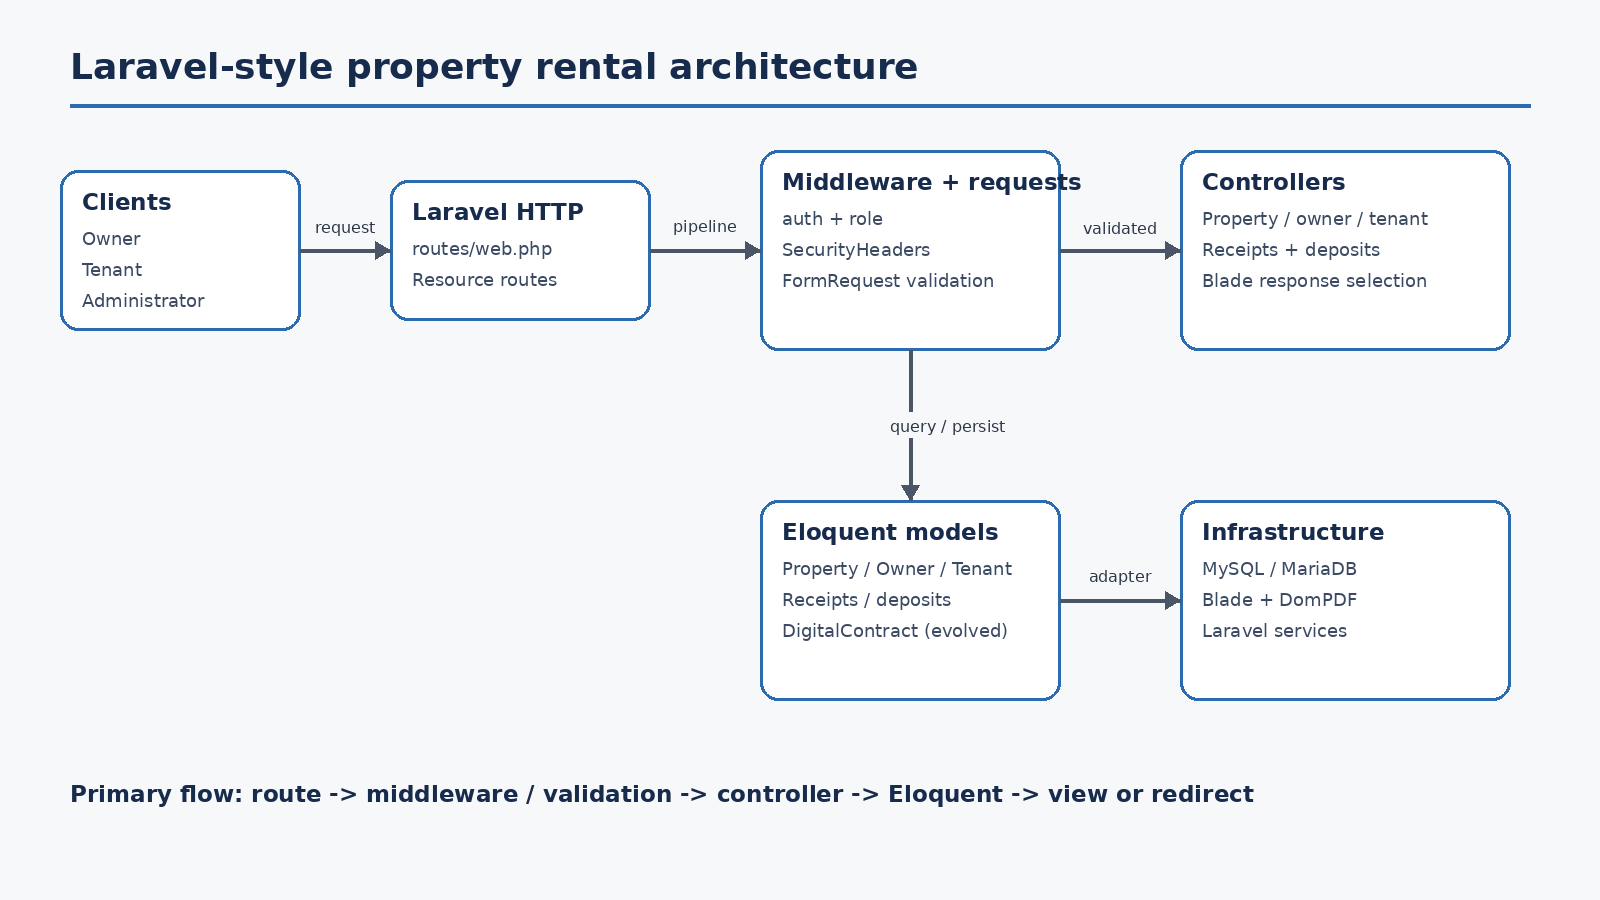
\includegraphics[width=\textwidth]{Part1/diagrams/architecture.png}
\caption{Laravel-style layers and the primary request flow. Editable source: \texttt{architecture.puml}.}
\end{figure}

A request traverses Laravel's global and route middleware, reaches a resource controller, invokes Eloquent Active Record models, and selects a Blade view or redirect response. \codepath{RoleMiddleware} can stop unauthorized requests while \codepath{SecurityHeaders} decorates downstream responses. CH01 adds a container-bound pricing Strategy, CH02 lets \codepath{PropertyController} compose filtering Specifications, and CH03 adds a State-driven contract domain object plus Eloquent persistence.

\subsection{Environment and execution}

Laravel dependencies were resolved in the \codepath{composer:2} container to Laravel 12.53.0; syntax and focused domain checks ran in \codepath{php:8.3-cli}. Part 3 used OpenJDK 17.0.20.1, Python 3.12.3, Node.js 24.14.1, and G++ 13.3.0 with C++20. Exact commands, versions, timing rules, and limitations are recorded in \codepath{README.md} and \codepath{Part3/evidence/environment_versions.txt}.

\section{Part 1 - Pattern discovery}

\subsection{Method}

Discovery was performed against the recorded public commit, not README claims alone. Controllers, Eloquent models, middleware, form requests, service-provider configuration, routes, and Blade views were inspected. Each candidate required recognizable participant roles and an observed call or framework lifecycle. Framework-origin participants are named explicitly. Absence is also evidence: direct Eloquent calls reject a Repository claim, the unused \codepath{Notifiable} trait does not establish an Observer collaboration, and no baseline algorithm family establishes Strategy.

\subsection{Baseline totals}

\begin{tabularx}{\textwidth}{Xr}
\toprule
\rowcolor{B4Blue}\color{white}\textbf{Measure} & \color{white}\textbf{Baseline}\\
\midrule
Distinct confirmed pattern types & 5\\
Confirmed pattern instances & 5\\
Concrete participant classes in mapped roles & 18\\
Unique mapped participant symbols & 15\\
Rejected candidates & 3\\
Uncertain candidates & 0\\
\bottomrule
\end{tabularx}

Concrete participant counts are per collaboration; unique-symbol counts remove overlaps. The authoritative row-level inventory is \codepath{data/patterns.csv}. Count logic and every cumulative snapshot are in \codepath{data/pattern_counts.csv}.

\subsection{Pattern inventory}

\begin{longtable}{p{0.20\textwidth}p{0.33\textwidth}p{0.10\textwidth}p{0.25\textwidth}}
\toprule
\rowcolor{B4Blue}\color{white}\textbf{Pattern type} & \color{white}\textbf{Instance} & \color{white}\textbf{Count} & \color{white}\textbf{Variable concrete roles}\\
\midrule
Model-View-Controller & Property Management Request Coordination & 1 & Resource controller, Eloquent models, Blade views.\\
Active Record & Property and Rental Record Persistence & 1 & \codepath{Property}, \codepath{Owner}, \codepath{Tenant}, receipt models.\\
Chain of Responsibility & Authentication and Security Pipeline & 1 & \codepath{RoleMiddleware}, \codepath{SecurityHeaders}, framework auth handler.\\
Template Method & Form Request Validation Lifecycle & 1 & Store/update request subclasses override lifecycle hooks.\\
Facade & Tenant Registration Infrastructure Access & 1 & Laravel \codepath{DB} and \codepath{Hash} facades.\\
\bottomrule
\end{longtable}

\begin{figure}[htbp]
\centering
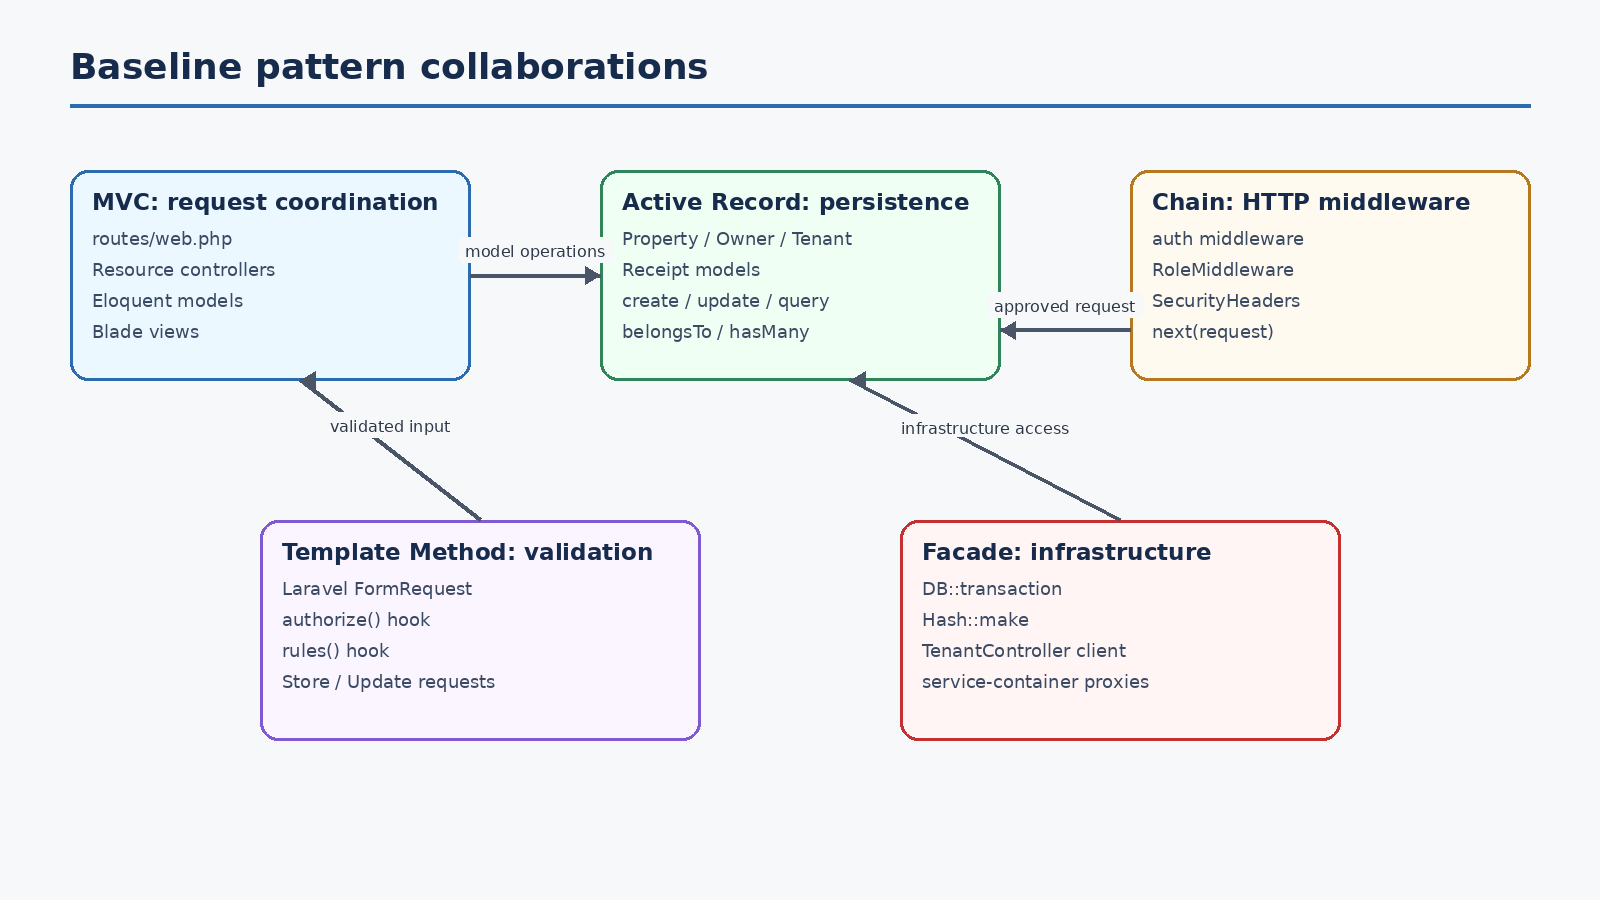
\includegraphics[width=\textwidth]{Part1/diagrams/baseline_patterns.png}
\caption{Baseline collaborations. Editable source: \texttt{baseline\_patterns.puml}.}
\end{figure}

\subsection{Instance 1: Property Management Request Coordination - MVC}

\textbf{Category and origin.} Architecture pattern; application structure using Laravel framework conventions.

\textbf{Participants.} Controller = \codepath{PropertyController} (lines 11--119). Models = \codepath{Property}, \codepath{Owner}, and \codepath{Tenant}. Views = the four templates under \codepath{resources/views/properties}. Router = resource registration in \codepath{routes/web.php}.

\textbf{Evidence.} The index action queries the model and selects \codepath{properties.index}; create, store, show, edit, update, and destroy follow the same request-controller-model-view separation.

\lstinputlisting[language=PHP,firstline=11,lastline=28]{Part1/code/app/Http/Controllers/PropertyController.php}

\textbf{Verification.} The route file, controller actions, Eloquent model, and actual Blade templates jointly confirm the collaboration; no View class is invented.

\subsection{Instance 2: Property and Rental Record Persistence - Active Record}

\textbf{Category and origin.} Enterprise data-source pattern; Laravel Eloquent framework plus application models.

\textbf{Participants.} Active Records = \codepath{Property}, \codepath{Owner}, \codepath{Tenant}, and receipt models. Mapping base = \codepath{Illuminate\Database\Eloquent\Model}. Relationships are declared with \codepath{belongsTo} and \codepath{hasMany}; controllers call static query and instance persistence methods.

\textbf{Evidence.} \codepath{Property} declares fillable attributes, casts, and relationship methods, while \codepath{PropertyController} directly calls \codepath{Property::create}, query builders, \codepath{update}, and \codepath{delete}.

\lstinputlisting[language=PHP,firstline=8,lastline=47]{Part1/code/app/Models/Property.php}

\textbf{Verification.} The model inheritance and direct persistence calls confirm Active Record. This same evidence rejects a separate application Repository pattern.

\subsection{Instance 3: HTTP Authentication and Security Pipeline - Chain of Responsibility}

\textbf{Category and origin.} GoF Behavioral / framework pipeline; Laravel and application middleware.

\textbf{Participants.} Handler = Laravel middleware contract and closure. Concrete handlers = framework \codepath{auth}, application \codepath{RoleMiddleware}, and \codepath{SecurityHeaders}. Client/configuration = route groups in \codepath{routes/web.php} and middleware registration in \codepath{bootstrap/app.php}.

\textbf{Evidence.} \codepath{RoleMiddleware} returns a redirect or 403 to stop the chain, otherwise calls \codepath{\$next(\$request)}. \codepath{SecurityHeaders} calls the next handler first and then decorates its response.

\lstinputlisting[language=PHP,firstline=23,lastline=34]{Part1/code/app/Http/Middleware/RoleMiddleware.php}

\textbf{Verification.} The route groups show ordered use of \codepath{auth} and role checks, while the middleware bodies expose pass/stop behavior.

\subsection{Instance 4: Form Request Validation Lifecycle - Template Method}

\textbf{Category and origin.} GoF Behavioral / framework lifecycle; Laravel base class with application hook implementations.

\textbf{Participants.} Abstract template = Laravel \codepath{FormRequest}. Primitive hook operations = \codepath{authorize} and \codepath{rules}. Concrete classes include \codepath{StorePropertyRequest}, \codepath{StoreTenantRequest}, and \codepath{StoreRentReceiptRequest}.

\textbf{Evidence.} Laravel owns resolution, authorization, validation, and controller invocation. Each application subclass supplies only its authorization decision and validation-rule map.

\lstinputlisting[language=PHP,firstline=7,lastline=27]{Part1/code/app/Http/Requests/StorePropertyRequest.php}

\textbf{Verification.} Multiple request subclasses repeat the same two hook signatures while controllers receive already validated request objects.

\subsection{Instance 5: Tenant Registration Infrastructure Access - Facade}

\textbf{Category and origin.} GoF Structural as implemented by Laravel's service-container facades.

\textbf{Participants.} Facades = \codepath{DB} and \codepath{Hash}. Hidden subsystems = Laravel database manager/connection and hashing manager. Client = \codepath{TenantController}.

\textbf{Evidence.} Tenant creation uses \codepath{DB::transaction} and \codepath{Hash::make} without locating or constructing the underlying services.

\lstinputlisting[language=PHP,firstline=28,lastline=45]{Part1/code/app/Http/Controllers/TenantController.php}

\textbf{Verification.} Imports and static proxy calls map directly to Laravel facade participants; the controller remains the client.

\subsection{Rejected candidates}

\begin{itemize}[leftmargin=*]
\item \textbf{Repository}: rejected at baseline because controllers query and mutate Eloquent Active Records directly; no application repository interface or adapter exists.
\item \textbf{Strategy}: rejected at baseline because no interchangeable application algorithm family and context are declared. CH01 deliberately introduces it.
\item \textbf{Observer}: rejected at baseline because \codepath{User} using Laravel's \codepath{Notifiable} trait is capability only; the application registers no event/listener or observer collaboration.
\end{itemize}

\section{Part 2 - Software evolution and refactoring}

\subsection{Evolution overview}

\begin{figure}[htbp]
\centering
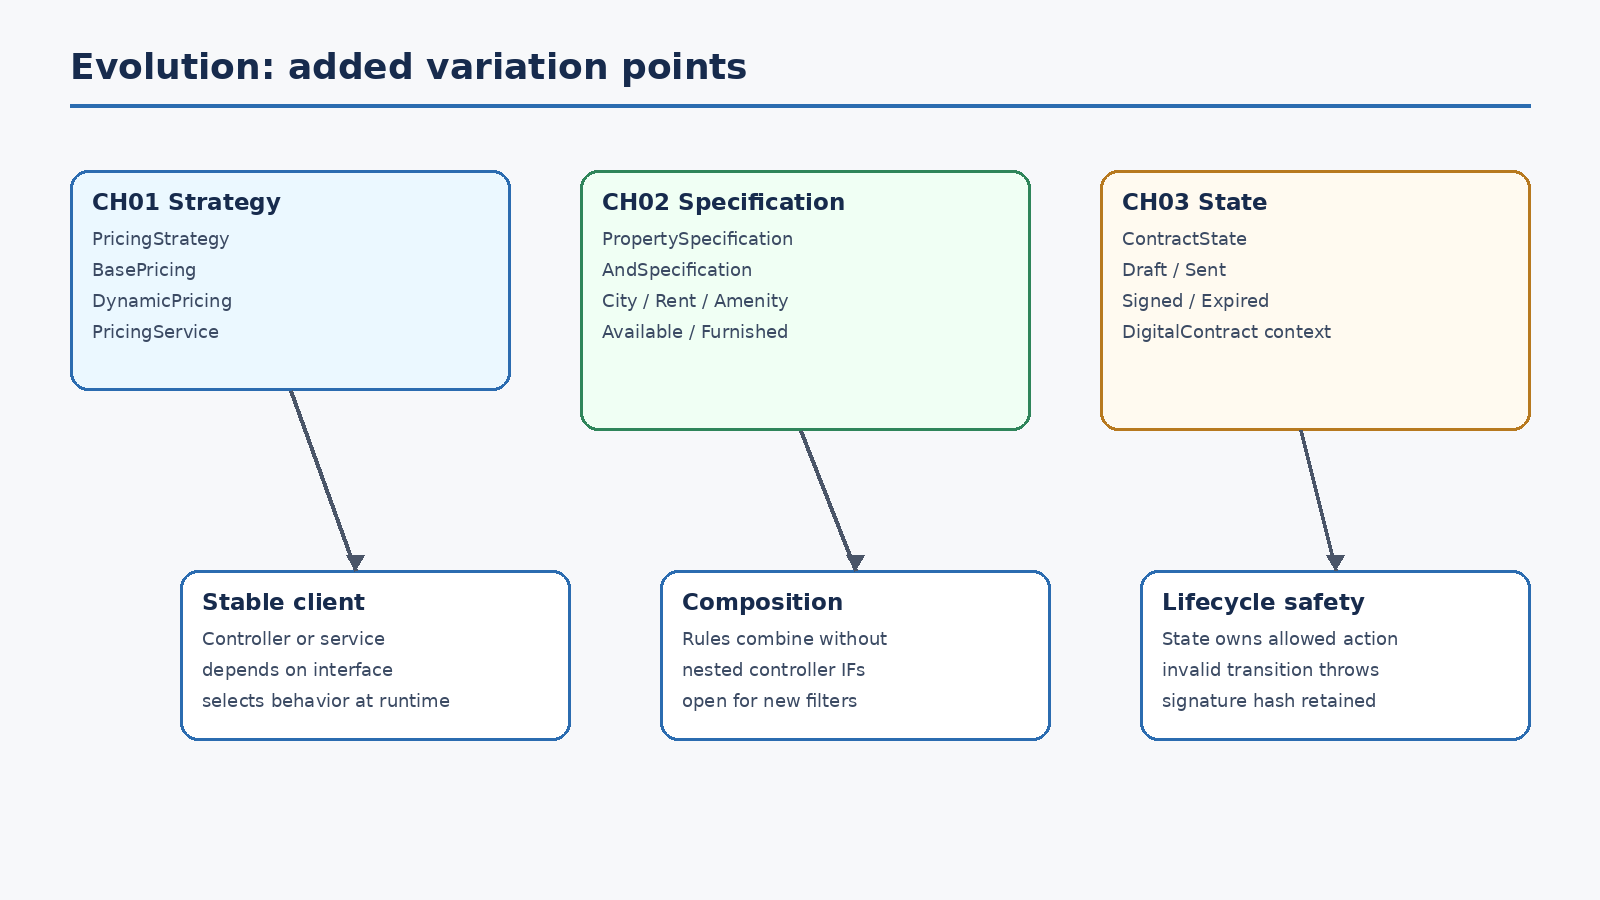
\includegraphics[width=\textwidth]{Part2/diagrams/evolved_patterns.png}
\caption{Three new variation points. Editable source: \texttt{evolved\_patterns.puml}.}
\end{figure}

\begin{figure}[htbp]
\centering
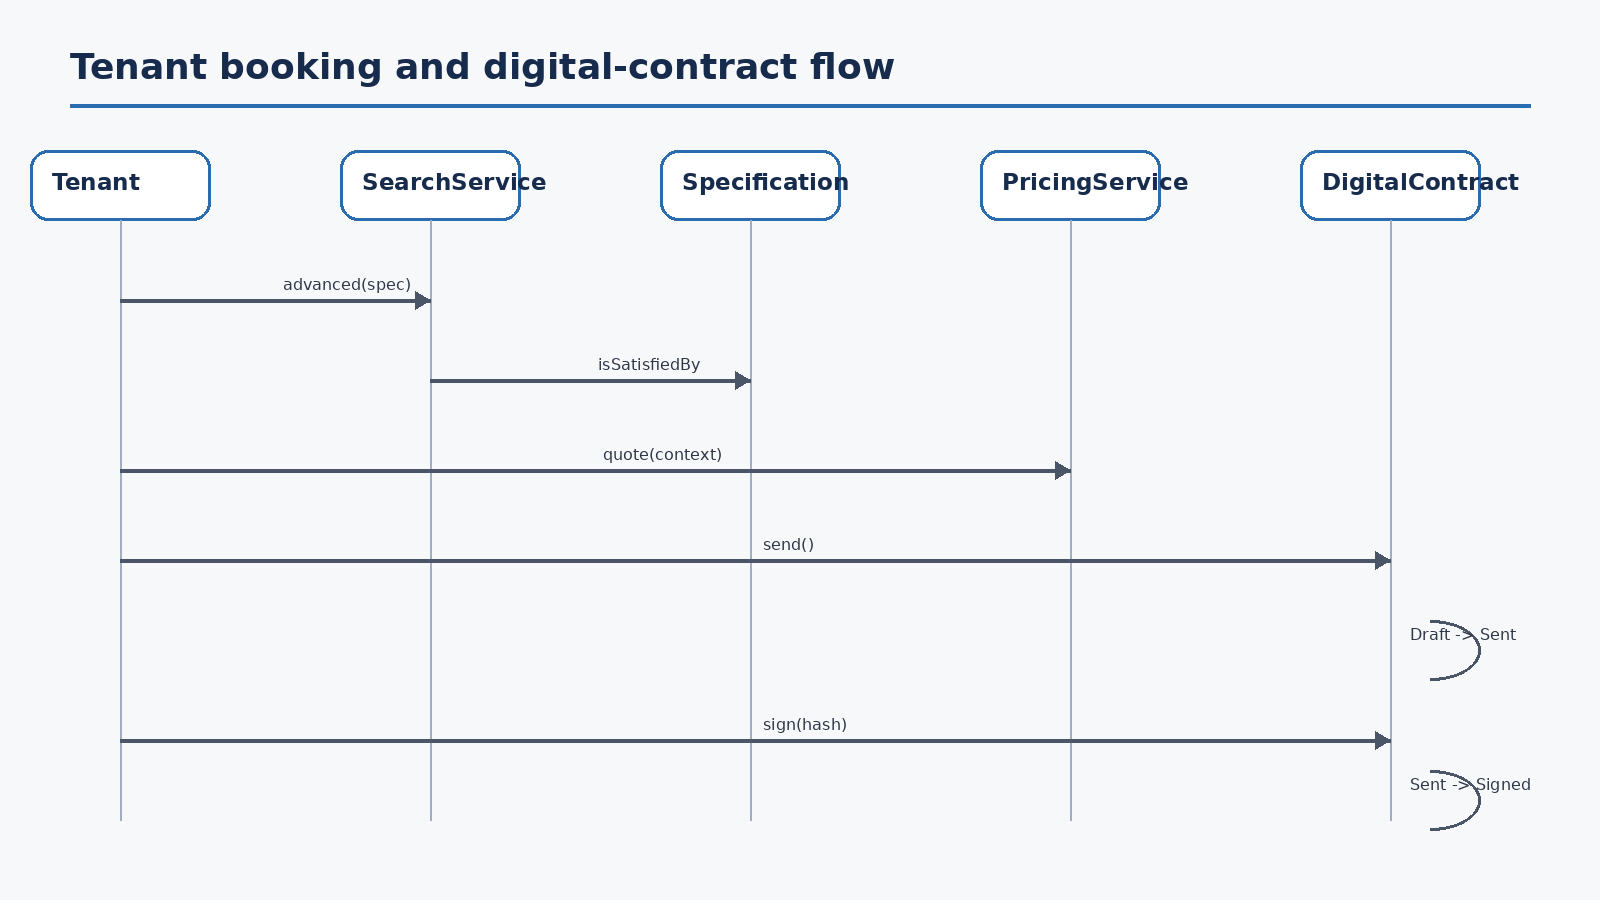
\includegraphics[width=\textwidth]{Part2/diagrams/evolution_sequence.png}
\caption{Search, quote, and contract-signing flow. Editable source: \texttt{evolution\_sequence.puml}.}
\end{figure}

\subsection{CH01 - Dynamic pricing}

\textbf{Requirement and acceptance criteria.} The application must select base or dynamic pricing without changing the quoting client. Peak months 4, 5, and 12 add 20 percent; occupancy of at least 0.80 adds 10 percent; leases of at least 12 months subtract 5 percent; adjustments are additive and rounded to two decimals. Invalid month, occupancy, or duration values must fail.

\textbf{Before.} \codepath{RentReceiptController::store} accepts a submitted amount directly; there is no pricing variation point.

\textbf{After.} Strategy = \codepath{PricingStrategy}. ConcreteStrategy = \codepath{BasePricing} and \codepath{DynamicPricing}. Context = \codepath{PricingService}. Parameter Object = \codepath{PricingContext}. \codepath{AppServiceProvider} binds the interface to \codepath{DynamicPricing}; \codepath{RentReceiptController} calls the service when dynamic pricing is requested.

\lstinputlisting[language=PHP,firstline=9,lastline=24]{Part2/code/app/Domain/Pricing/DynamicPricing.php}

\textbf{Refactoring analysis.} Extract Strategy removes the pressure to grow one quote method with plan-type conditionals. Introduce Parameter Object groups three correlated, validated inputs. New algorithms can implement \codepath{PricingStrategy}; existing clients continue calling \codepath{quote}. The cost is more classes and a runtime-selection responsibility.

\textbf{Tests and evidence.} The focused PHP runner checks base and combined dynamic results; the cross-language suite covers six shared cases per language. Commit: \codepath{7e9bd9ded113e91cca10e727a7eeff29c88d0ed8}. Patch: \codepath{Part2/changes/CH01/dynamic_pricing.patch}. Pattern effect: Strategy newly introduced.

\subsection{CH02 - Advanced property filtering}

\textbf{Requirement and acceptance criteria.} Availability, case-insensitive city, inclusive rent range, amenity, and furnished rules must run alone or as an AND composite. The shared fixture must return only property id 1 for the five-rule composite. An inverted range must fail. Adding a rule must not require editing existing rules.

\textbf{Before.} \codepath{PropertyController::index} offers only a latest-first paginated listing. Adding several optional filters directly would create a growing conditional query-construction method.

\textbf{After.} Specification = \codepath{PropertySpecification}. CompositeSpecification = \codepath{AndSpecification}. Concrete specifications cover availability, city, rent range, amenity, furnishing, address, maximum rent, and status. \codepath{PropertyFilterService} evaluates the abstraction, and \codepath{PropertyController} composes request-driven address, rent, and status rules.

\lstinputlisting[language=PHP,firstline=5,lastline=22]{Part2/code/app/Domain/Search/AndSpecification.php}

\textbf{Refactoring analysis.} Replace Conditional with Polymorphism moves independent predicates into named rule objects. Composite makes conjunction explicit and recursive. The Open/Closed benefit is practical: a new rule class can be combined without changing existing rule implementations. The trade-off is allocation and discoverability across more small classes; large data stores would translate specifications to database queries rather than filter every object in memory.

\textbf{Tests and evidence.} The PHP runner applies the shared five-rule fixture and returns only property id 1. Cross-language suites also check reusable single rules and invalid ranges. Commit: \codepath{2b2dd6246dd50f4a53a991e5429b22da1b1a5c4f}. Patch: \codepath{Part2/changes/CH02/advanced_filtering.patch}. Pattern effect: Specification newly introduced.

\subsection{CH03 - Digital contract management}

\textbf{Requirement and acceptance criteria.} A contract begins Draft. Only Draft can be sent. Sent can be signed or expired. Signed and Expired are terminal. Document and signature identities use 64-character lowercase SHA-256 hashes. An invalid hash or transition must fail.

\textbf{Before.} The public baseline has property occupancy and receipt records but no dedicated lease or digital-contract entity, signature evidence, or transition ownership.

\textbf{After.} State = \codepath{ContractState}. AbstractState = \codepath{AbstractContractState}, whose defaults reject all operations. Concrete states = \codepath{DraftState}, \codepath{SentState}, \codepath{SignedState}, and \codepath{ExpiredState}. Context = domain \codepath{DigitalContract}. A separate Eloquent \codepath{Models/DigitalContract} and migration persist property, tenant, hashes, and status.

\lstinputlisting[language=PHP,firstline=22,lastline=66]{Part2/code/app/Domain/Contracts/DigitalContract.php}

\textbf{Refactoring analysis.} Replace State-Dependent Conditional with State objects prevents a central status switch from expanding with every action. Each state owns allowed behavior; the abstract base makes denial the default. This improves transition locality but adds classes. The educational implementation stores integrity identifiers only. It does not provide signer identity, public-key validation, timestamping, non-repudiation, encryption, retention, or jurisdiction-specific e-signature compliance.

\textbf{Tests and evidence.} The PHP runner checks Draft $\rightarrow$ Sent $\rightarrow$ Signed, stored signature hash, blocked expiry of a signed contract, and invalid hash rejection. Commit: \codepath{8e2af082067bb83aab7e40caf2b7a463fef8b643}. Patch: \codepath{Part2/changes/CH03/digital_contract.patch}. Pattern effect: State newly introduced.

\subsection{Before/after metrics and interpretation}

\begin{longtable}{p{0.18\textwidth}rrrrrr}
\toprule
\rowcolor{B4Blue}\color{white}\textbf{Snapshot} & \color{white}\textbf{Prod LOC} & \color{white}\textbf{Test LOC} & \color{white}\textbf{Tests} & \color{white}\textbf{Types} & \color{white}\textbf{Instances} & \color{white}\textbf{Concrete}\\
\midrule
Original code & 2055 & 27 & 1/2 & 5 & 5 & 18\\
After CH01 & 2143 & 27 & 2/2 & 6 & 6 & 21\\
After CH02 & 2303 & 27 & 4/4 & 7 & 7 & 32\\
After CH03 & 2450 & 120 & 10/10 & 8 & 8 & 38\\
\bottomrule
\end{longtable}

Every LOC value is directly measured from the corresponding preserved local commit using the same rule: nonblank, noncomment physical PHP lines under \codepath{app/}, excluding tests and dependencies. The baseline's 1/2 is reported honestly: its stock feature test expects 200 while its root route intentionally redirects to login. Change-level acceptance counts cover the introduced behavior; the final snapshot also passes the corrected 2/2 Laravel suite. Improvement evidence is localized variation, composable rules, explicit transitions, integration points, and passing acceptance behavior - not LOC growth by itself.

All five baseline collaborations remain. CH01 introduces the sixth type, Strategy; CH02 introduces the seventh, Specification; CH03 introduces the eighth, State, while extending Active Record with contract persistence. Final totals are eight types and eight instances. The complete version-by-version inventory is \codepath{data/patterns_evolution.csv}.

\section{Part 3 - Cross-language analysis}

\subsection{Selected patterns and common specifications}

Dynamic Rent Pricing (Strategy) and Advanced Property Filtering (Specification) were selected because both changes isolate volatile business rules and require composition/substitution across a stable client. State was not selected because the user request specifies two significant patterns.

\textbf{Strategy fixture.} Base rent is 1000. Base strategy returns 1000. Dynamic cases expect 1200 for peak only, 1100 for occupancy only, 1250 for peak plus occupancy minus long-stay discount, and 950 for long stay only. Month 13 must fail.

\textbf{Specification fixture.} Four properties vary by city, rent, availability, amenities, and furnishing. A composite of available + Kochi + rent 18000--25000 + parking + furnished returns only id 1. City alone returns three, available alone returns three, and an inverted range fails.

\subsection{Actual results and static/dynamic comparison}

\begin{longtable}{p{0.14\textwidth}p{0.14\textwidth}rrp{0.18\textwidth}rp{0.23\textwidth}}
\toprule
\rowcolor{B4Blue}\color{white}\textbf{Pattern} & \color{white}\textbf{Language} & \color{white}\textbf{LOC} & \color{white}\textbf{Max CC} & \color{white}\textbf{Runtime/compiler} & \color{white}\textbf{Median ms} & \color{white}\textbf{Result}\\
\midrule
Strategy & Java & 38 & 4 & OpenJDK 17.0.20.1 & 64 & 6/6 passed\\
Strategy & Python & 35 & 4 & Python 3.12.3 & 43 & 6/6 passed\\
Strategy & JavaScript & 33 & 4 & Node.js 24.14.1 & 36 & 6/6 passed\\
Strategy & C++ & 42 & 4 & G++ 13.3.0 C++20 & 11 & 6/6 passed\\
Specification & Java & 33 & 2 & OpenJDK 17.0.20.1 & 68 & 5/5 passed\\
Specification & Python & 44 & 2 & Python 3.12.3 & 46 & 5/5 passed\\
Specification & JavaScript & 26 & 2 & Node.js 24.14.1 & 37 & 5/5 passed\\
Specification & C++ & 62 & 2 & G++ 13.3.0 C++20 & 11 & 5/5 passed\\
\bottomrule
\end{longtable}

The timing protocol compiles first, performs one warmup, then measures five complete test processes on the same machine and reports the median. It includes startup and fixture assertions. The samples are preserved at \codepath{Part3/evidence/cross_language_runs.txt}; they do not support a claim that one language is generally faster.

\subsection{Language comparison}

\begin{longtable}{p{0.14\textwidth}p{0.19\textwidth}p{0.27\textwidth}p{0.30\textwidth}}
\toprule
\rowcolor{B4Blue}\color{white}\textbf{Language} & \color{white}\textbf{Abstraction} & \color{white}\textbf{Composition / ownership} & \color{white}\textbf{Observed trade-off}\\
\midrule
Java & Nominal interfaces and records & Strategy held by a service; Specification composite holds a list of interfaces. & Strong role visibility and immutable record fixtures; more declarations than JavaScript.\\
Python & Structural \codepath{Protocol} plus dataclasses & Ordinary object references; tuple-backed composite. & Concise immutable data and readable rules; interface conformance is primarily tooling/static-checker knowledge at authoring time.\\
JavaScript & Duck-typed classes & Strategy and rule objects share method shape without a nominal interface. & Smallest Specification LOC and direct composition; misspelled roles fail only when exercised.\\
C++ & Abstract virtual base classes & \codepath{unique_ptr} for replaceable Strategy; \codepath{shared_ptr} for heterogeneous retained rules. & Ownership is explicit and startup here is small after compilation; templates or value erasure could reduce virtual allocation at higher complexity.\\
\bottomrule
\end{longtable}

Despite syntax differences, the pattern structure is stable. Strategy keeps the context independent of a replaceable algorithm. Specification gives every predicate the same test operation and lets a composite hold other specifications. This structural equivalence, identical inputs, and identical outputs are stronger evidence than matching class names alone.

\section{LLM records and human verification}

Eight prompt records provide two records for each named team member. Each record has an exact prompt, a saved output, and a verification file. They cover baseline discovery/challenge, dynamic pricing/metrics, advanced filtering/language comparison, and digital contracts/dataset audit. The normalized index is \codepath{data/llm.csv}; files are under \codepath{prompts/}.

The records are labeled as OpenAI Codex draft runs and updated against the public baseline on 11 October 2026. They are technically checked against source, tests, and datasets, but they are not falsely presented as independently typed by each student. Every verification form therefore contains a pending member-acknowledgement line. The team must inspect and sign those records before submission.

\begin{longtable}{p{0.22\textwidth}p{0.26\textwidth}p{0.34\textwidth}p{0.10\textwidth}}
\toprule
\rowcolor{B4Blue}\color{white}\textbf{Member} & \color{white}\textbf{Technical scope} & \color{white}\textbf{Automated verification} & \color{white}\textbf{Share}\\
\midrule
Earlapally Sahith Siddarth & Public-source selection, architecture and baseline discovery & Exact baseline commit; five mapped rows & 25\%\\
Kankanala Sanithya Reddy & Dynamic pricing and Strategy metrics & Pricing checks; Strategy 6/6 in four languages & 25\%\\
Eati Manoj & Advanced filtering and cross-language Specification & Specification 5/5 in four languages & 25\%\\
Bussa Surya & Digital contracts, dataset audit, final integration & Contract checks; 2/2 Laravel suite; CSV reconciliation & 25\%\\
\bottomrule
\end{longtable}

Human verification remains a mandatory final activity. \codepath{HUMAN_VERIFICATION.md} provides a team declaration and one signature/date field per member. Automated execution cannot verify authorship or institutional approval.

\section{Dataset, metrics, and audit trail}

The workbook \codepath{data/B4_Dataset.xlsx} mirrors seven authoritative CSV files. Its Summary sheet uses formulas to show five baseline instances, eight final instances, eight final types, 2,450 final production LOC, 395 added production LOC, 10 focused evolution checks, and 100 percent contribution allocation. Separate sheets preserve Patterns, Pattern Counts, Evolution, Cross Language, LLM Records, Metrics, and Contributions.

The CSV files use UTF-8, one header row, relative paths from \codepath{B4/}, and quoted comma-containing fields. The static metric script is \codepath{tools/metrics.py}. Source and test output are preserved as raw evidence rather than copied only into prose.

\section{Findings and limitations}

\begin{enumerate}[leftmargin=*]
\item The most defensible baseline patterns are collaborations visible in the recorded public source. Rejecting Repository, Strategy, and Observer at baseline avoids promoting framework vocabulary or capability traits into unsupported instances.
\item Framework and application participants coexist. MVC, Active Record, middleware Chain of Responsibility, Form Request Template Method, and Facade explain the original Laravel design; Strategy, Specification, and State explain the introduced variation points.
\item The three changes increase class count deliberately. The benefit is that new pricing rules, search predicates, and contract states have named extension points and localized tests.
\item Cross-language syntax changes, but participant responsibilities and fixtures can remain constant. This makes pattern-level comparison more meaningful than raw LOC alone.
\item The evolved code is an academic change set, not a production deployment. Digital-contract evidence is hash-based and does not provide identity proof, PKI validation, trusted timestamps, non-repudiation, retention policy, or jurisdiction-specific compliance.
\item Timing results describe this machine and startup-heavy micro-tests. They do not rank languages generally.
\end{enumerate}

\section{Submission readiness}

The deliverable contains one B4 team folder with one report, source snapshots, diagrams, tests, prompts, CSVs, and one Excel workbook. Before opening the pull request, the team must:

\begin{enumerate}[leftmargin=*]
\item obtain and record faculty approval for the selected public application;
\item sign the central and per-prompt verification forms;
\item upload only \codepath{B4/} to the team's fork of the course repository;
\item commit the folder and record the final submission commit;
\item open one pull request titled \textbf{B4: Final submission} to the original repository's \codepath{main} branch and record its URL.
\end{enumerate}

\section{References}

\begin{enumerate}[leftmargin=*]
\item E. Gamma, R. Helm, R. Johnson, and J. Vlissides, \emph{Design Patterns: Elements of Reusable Object-Oriented Software}, Addison-Wesley, 1994.
\item Mohsin Rafique, \emph{Property Management}, \url{https://github.com/mohsin-rafique/property-management}, commit \codepath{f127b4e218018715586a52cede08e182ca45c983}, MIT License, accessed 2026-10-11.
\item Laravel 12 Documentation, \url{https://laravel.com/docs/12.x}, accessed 2026-10-11.
\item Laravel 12 Eloquent ORM, \url{https://laravel.com/docs/12.x/eloquent}, accessed 2026-10-11.
\item Laravel 12 Middleware, \url{https://laravel.com/docs/12.x/middleware}, accessed 2026-10-11.
\item PHP Manual, Object Interfaces, \url{https://www.php.net/manual/en/language.oop5.interfaces.php}, accessed 2026-10-11.
\item Team B4 changes, tests, raw timings, SHA-256 manifests, and normalized datasets included with this report.
\end{enumerate}

\appendix
\section{Evidence index}

\small
\begin{longtable}{p{0.39\textwidth}p{0.51\textwidth}}
\toprule
\rowcolor{B4Blue}\color{white}\textbf{Path} & \color{white}\textbf{Purpose}\\
\midrule
\codepath{Part1/evidence/test_results.txt} & Unchanged public baseline result: 1 passed, 1 stale example expectation failed.\\
\codepath{Part2/evidence/test_results.txt} & Evolved Laravel result: 2/2; focused evolution result: 10/10.\\
\codepath{Part3/evidence/cross_language_runs.txt} & Five timing samples and result output for eight implementations.\\
\codepath{Part1/evidence/source_manifest.sha256} & Integrity manifest for the baseline snapshot.\\
\codepath{Part2/evidence/source_manifest.sha256} & Integrity manifest for the evolved snapshot.\\
\codepath{Part2/changes/CH01..CH03} & Acceptance notes and unified source patches.\\
\codepath{data/patterns.csv} & Baseline pattern-to-source mapping.\\
\codepath{data/patterns_evolution.csv} & Per-snapshot status and participant evolution.\\
\codepath{data/cross_language.csv} & LOC, CC, runtime, command, result, median, and language notes.\\
\codepath{data/llm.csv} & Exact prompt/input/output/evaluation/verification index.\\
\codepath{data/B4_Dataset.xlsx} & Formatted Excel view of all normalized data.\\
\codepath{HUMAN_VERIFICATION.md} & Required final human sign-off.\\
\bottomrule
\end{longtable}
\normalsize

\section{Folder structure}

\begin{lstlisting}[basicstyle=\ttfamily\tiny]
B4/
  README.md
  HUMAN_VERIFICATION.md
  B4_Report.tex
  B4_Report.pdf
  data/
    patterns.csv, pattern_counts.csv, patterns_evolution.csv
    cross_language.csv, llm.csv, metrics.csv, contributions.csv
    B4_Dataset.xlsx
  Part1/ code/, diagrams/, evidence/, llm/
  Part2/ code/, changes/CH01..CH03/, diagrams/, evidence/, llm/
  Part3/ strategy/, filter_specification/, evidence/, llm/, run_all.sh
  prompts/ two prompt-output-verification records per member
  tools/ metrics, diagram, and workbook builders
\end{lstlisting}

\end{document}
